% !Mode\dots ``TeX:UTF-8''
% !TEX root = ../bare_jrnl.tex

\section{Preliminaries} 
\label{sec:pre}
We now introduce the formal definition of {\BCNs} and its control theoretical properties. Throughout the paper, we use $\mathbb{B}$ to denote the set of Boolean values $\{0,1\}$ and $\mathbb{T}$ to denote the set of discrete time domain represented by the set of  natural numbers.

\subsection{Boolean Control Networks}

We take the definition in ~\cite{Ideker2001A} in which a Boolean control network (\BCN)  is given a directed graph together with two  Boolean valued functions which define the updating rules for the  values of the nodes. 

\begin{definition}[Boolean Control Network] 
\label{def:BCN}
A \BCN\ is a tuple $\BB = (I,S,O, E, \sigma, \rho)$, where 
\begin{itemize}
\item $I$, $S$ and $O$ are three finite nonempty disjoint sets of nodes (or vertices)
\begin{itemize}
	\item {\bf input nodes} $I=\{\mathsf{i}_1$,\ldots ,$\mathsf{i}_{\ell}\}$
	\item {\bf state nodes}  $S= \{\mathsf{s}_1$,\ldots ,$\mathsf{s}_m\}$, and 
	\item {\bf output nodes}: $O= \{\mathsf{o}_1$,\ldots ,$\mathsf{o}_n\}$.
	\end{itemize}	
	Each node is a Boolean variable which can take values in $\mathbb{B}$.
\item  $E \subseteq ((I\cup S)\times S)\cup (S\times O)$ is a set of edges among the nodes, and we say node $v$ directly affects node  $v'$  when $(v,v')$ is an edge in $E$.
\item The Boolean valued functions $\sigma: \mathbb{B}^\ell\times  \mathbb{B}^m \mapsto \mathbb{B}^m$ and $\rho: \mathbb{B}^m\mapsto \mathbb{B}^n$ are functions from the pairs of $\ell$-dimension and $m$-dimension vectors  of Boolean values to  the $m$-dimension vectors Boolean values and from the  $m$-dimension vectors to the  $n$-dimension vectors  of Boolean values, respectively. 
%\item $\theta$ is a Boolean expression of the state nodes.
\item {\em Updating rules }:  We use 
 $\mathsf{i}= (\mathsf{i}_1,\ldots, \mathsf{i}_\ell)$, $\mathsf{s}= (\mathsf{s}_1,\ldots, \mathsf{s}_m)$ and $\mathsf{o}= (\mathsf{o}_1,\ldots, \mathsf{o}_n)$ to denote the three variables Boolean vectors corresponding  to the input nodes, state nodes and output nodes. At any time $t\in \mathbb{T}$ during the execution 
 of $\BB$, each of the variables  $\mathsf{i}$, $\mathsf{s}$ and $\mathsf{o}$  (thus each every node of $\BB$ too) take a vector of Boolean values $\mathsf{i}(t)$, $\mathsf{s}(t)$, $\mathsf{o}(t)$  in  $\mathbb{B}^\ell$, $\mathbb{B}^m$ and $\mathbb{B}^n$, respectively, such that the following equations are satisfied
\begin{equation}
\begin{split}
\mathsf{s}(t+1)=&\sigma(\mathsf{i}(t),\mathsf{s}(t))\\
\mathsf{o}(t)=&\rho(\mathsf{s}(t))
\end{split}
\label{equ:1}
\end{equation}
The above equations are also assumed to satisfy the following three conditions
\begin{enumerate}
%\item $\mathsf{s}(0)$ satisfies the initial condition $\theta$;
\item the value of $\mathsf{s}_k(t+1)$ in $\mathsf{s}(t+1)$ is affected by the value  $\mathsf{i}_j(t)$ of an input node $\mathsf{i}_j \in I$ (or by the value $\mathsf{s}_j(t)$ of a state node $\mathsf{s}_j\in S$) at time $t$ only when $(\mathsf{i}_j, \mathsf{s}_k)\in E$ (or $(\mathsf{s}_j, \mathsf{s}_k)\in E$, respectively); and
\item the value $\mathsf{o}_k(t)$ in $\mathsf{o}(t)$ of an output node $\mathsf{o}_k\in O$ is affected by the value $\mathsf{s}_j(t)$ of a state node $\mathsf{s}_j\in S$ only when $(\mathsf{s}_j,\mathsf{o}_k)\in E$.
\end{enumerate}
\end{itemize}

\end{definition}
 The two updating functions are called the  {\bf updating rules}  of $\BB$. They define the value of the state nodes at any time by the values of the inout nodes and state nodes at the previous time point, and the the values of the output nodes by the value of the state nodes, respectively. We use 
 \[\mathcal{I}_\BB=\{\mathsf{i}^0,\ldots,\mathsf{i}^{2^{l}-1} \},\] 
 \[\mathcal{S}_\BB=\{\mathsf{s}^0,\ldots,\mathsf{s}^{2^{m}-1}\},\] 
 \[ \mathcal{O}_\BB=\{\mathsf{o}^0,\ldots,\mathsf{o}^{2^{n}-1}\}\] to denote  the sets of all possible inputs, states and outputs of $\BB$, respectively. For instance if \[\mathsf{s}(t)=(\mathsf{s}_1(t)\mathsf{s}_2(t) \mathsf{s}_3(t) \mathsf{s}_4(t))=(0101),\] then %$\mathsf{s}(t)$ can be represented by 
 \[\mathsf{s}(t)=\mathsf{s}^{(0\times2^3+1\times2^2+0\times2^1+1\times2^0)}=\mathsf{s}^5.\] And we will omit the subscript $\BB$ of $\mathcal{I}_\BB$, $\mathcal{S}_\BB$ and $\mathcal{O}_\BB$ when there is no confusion. %Obviously, $\mathcal{I}_\BB$, and $\mathcal{S}_\BB$ and $\mathcal{O}_\BB$ are finite with $2^\ell$, $2^m$ and $2^n$ elements, respectively. 


\begin{figure}[!t]
      \centering
      \framebox{\parbox{3in}{
		\centerline{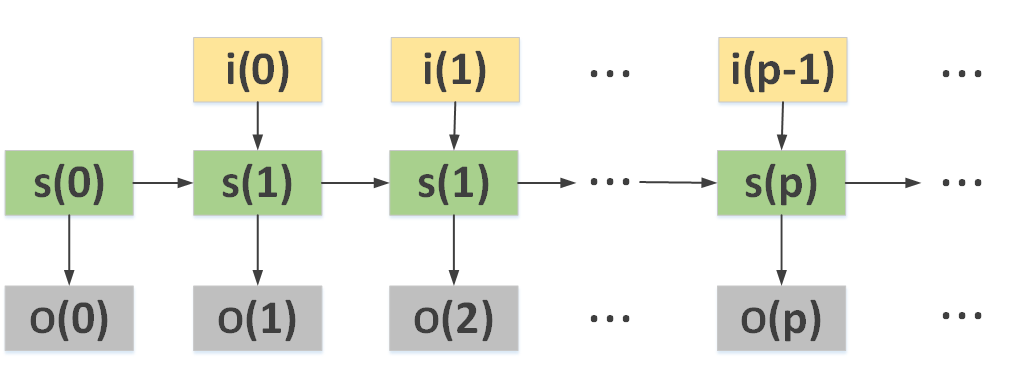
\includegraphics[scale=0.17]{figures/Fig10.png}}
	}}
      
      \caption{The relationship of inputs, states and outputs.}
      \label{fig:10}
  \end{figure}
%===========================================================
\begin{example}\label{exa:2}
	 \begin{figure}[thpb]
		\centering
		\framebox{\parbox{3in}{
				\centerline{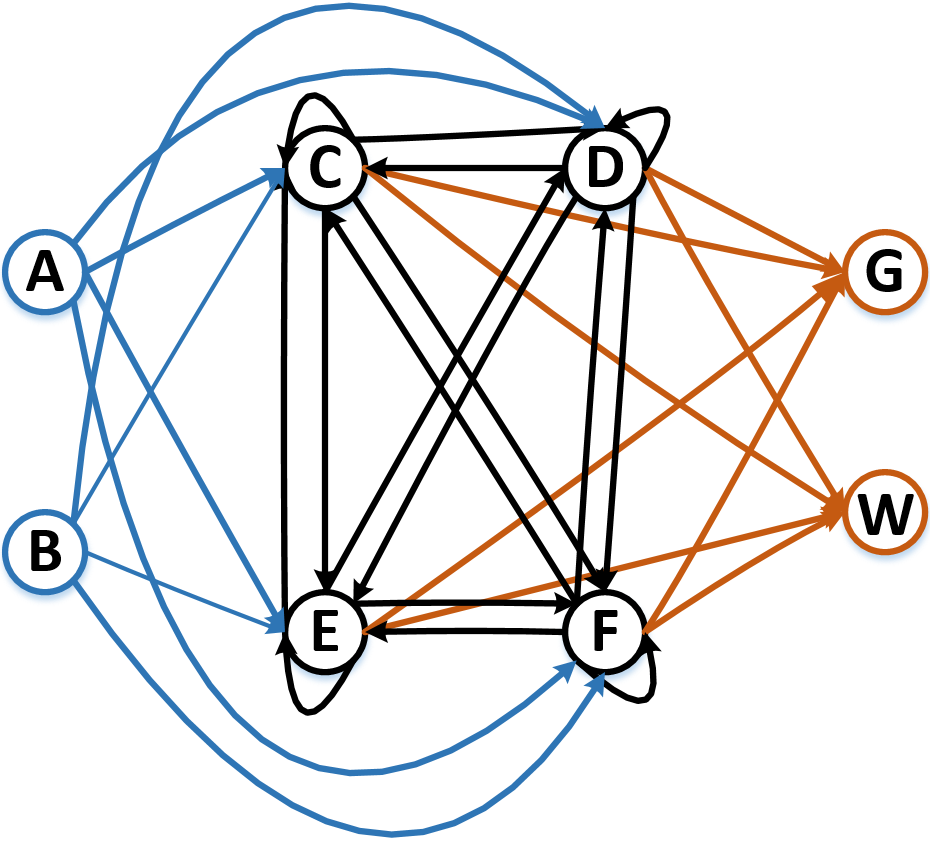
\includegraphics[scale=0.23]{figures/Fig1.png}}
		}}
		
		\caption{A Boolean control network. }%We use blue, black and orange, to distinguish three types of nodes and three types of edges. with two input-nodes $A$ and $B$, four state-nodes $C$, $D$, $E$ and $F$, and two output-nodes $G$, $W$.
		\label{fig:1}
	\end{figure}
%	
Let $\BB$ be the \BCN\  shown in Fig.~\ref{fig:1} which has two  input-nodes $I=\{\mathsf{i}_1,\mathsf{i}_2\}$ , four state-nodes $S=\{\mathsf{s}_1, \mathsf{s}_2,\mathsf{s}_3, \mathsf{s}_4\}$ and two output-nodes $O=\{\mathsf{o}_1,\mathsf{o}_2\}$. The set of edges $E$ and 
the updating rules $\sigma: \mathbb{B}^{2}\times \mathbb{B}^{4}\mapsto \mathbb{B}^4$ and $\rho:\mathbb{B}^4\mapsto \mathbb{B}^2$ are given in the truth table (Fig.~\ref{fig:2}) from which the updating rules in terms of logic functions can be easily recovered.   For instance, %from the truth table we have 
the updating rule of output-node $\mathsf{o}_1$ is 
$\mathsf{o}_1(t)=\mathsf{s}_1(t)\vee {({\mathsf{s}_2}(t)\wedge { \mathsf{s}_3}(t)\wedge {\mathsf{s}_4}(t))}$. 
%The set of all possible inputs $\mathcal{I}_\BB=\{\delta_{4}^0,\ldots,\delta_{4}^{3}\}$, the set of all states $\mathcal{S}_\BB=\{\delta_{16}^0,\ldots,\delta_{16}^{15}\}$ and the set of all outputs $\mathcal{O}_\BB=\{\delta_{4}^0,\ldots,\delta_{4}^{3}\}$.
 \begin{figure}[thpb]
	\centering
	\framebox{\parbox{3in}{
			\centerline{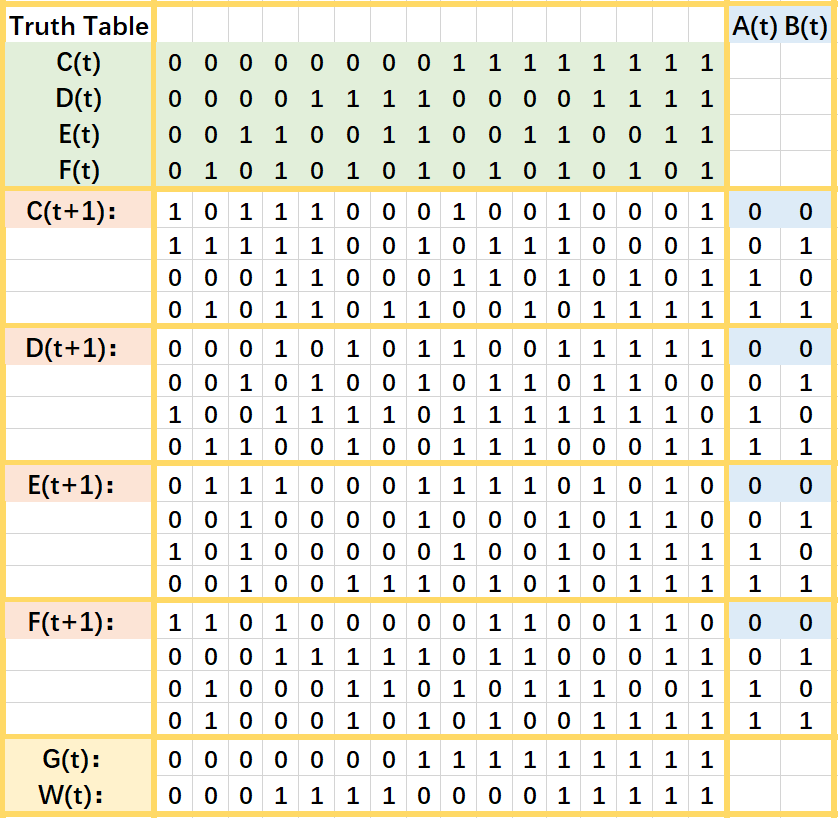
\includegraphics[scale=0.343]{figures/Fig2.png}}
	}}
	\caption{The truth table which describe the updating rules of the \BCN\ shown in Fig.~\ref{fig:1}.}
	\label{fig:2}
\end{figure}
%For instance, from the truth table we have the updating rule of output-node $G$ is 
%$G(t)=C(t)\vee {({D}(t)\wedge { E}(t)\wedge {F}(t))}.$
 %
\end{example}   

%===========================================================

%The reason why we use the truth table to describe the updating rules of the \BCN\ is that it would be more convenient for us to convert the $\mathsf{i}(t)$, $\mathsf{s}(t)$ and $\mathsf{o}(t)$ into their abbreviation forms. 
%That we use 
%\begin{itemize}
%  \item $\delta^i_{2^m}$ represents the abbreviation form of $\mathsf{i}(t)$, where $i=\sum_{x=1}^m \mathsf{i}_{x}(t)\times 2^{m-x}$;
%  \item $\delta^j_{2^n}$ represents the abbreviation form of $\mathsf{s}(t)$, where $j=\sum_{x=1}^n \mathsf{s}_{x}(t)\times 2^{n-x}$;
%  \item $\delta^w_{2^q}$ represents the abbreviation form of $\mathsf{o}(t)$, where  $w=\sum_{x=1}^q \mathsf{o}_{x}(t)\times 2^{q-x}$.
%\end{itemize}
%
%For instance if $\mathsf{s}(t)=\begin{bmatrix}\mathsf{s}_1(t)\\\mathsf{s}_2(t) \\ \mathsf{s}_3(t) \\\mathsf{s}_4(t)\end{bmatrix}=\begin{bmatrix}0\\1\\0\\1\end{bmatrix}$, then $\mathsf{s}(t)$ can be represented by $\delta^{(0\times2^3+1\times2^2+0\times2^1+1\times2^0)}_{2^4}=\delta^5_{16}$. 
%
%In the \BCN\ which shown in the Fig.~\ref{fig:1}, we consider 
%\begin{itemize}
%  \item $A(t)$ as $\mathsf{i}_{1}(t)$, $B(t)$ as $\mathsf{i}_{2}(t)$;
%  \item $C(t)$ as $\mathsf{s}_{1}(t)$, $D(t)$ as $\mathsf{s}_{2}(t)$;
%  \item $E(t)$ as $\mathsf{s}_{3}(t)$, $F(t)$ as $\mathsf{s}_{4}(t)$;
%  \item $G(t)$ as $\mathsf{o}_{1}(t)$, $W(t)$ as $\mathsf{o}_{2}(t)$.
%\end{itemize}
%
%Then, the updating rules which shown in Fig.~\ref{fig:2} can be represented by Fig.~\ref{fig:6}.
% \begin{figure}[thpb]
%      \centering
%      \framebox{\parbox{3in}{
%		\centerline{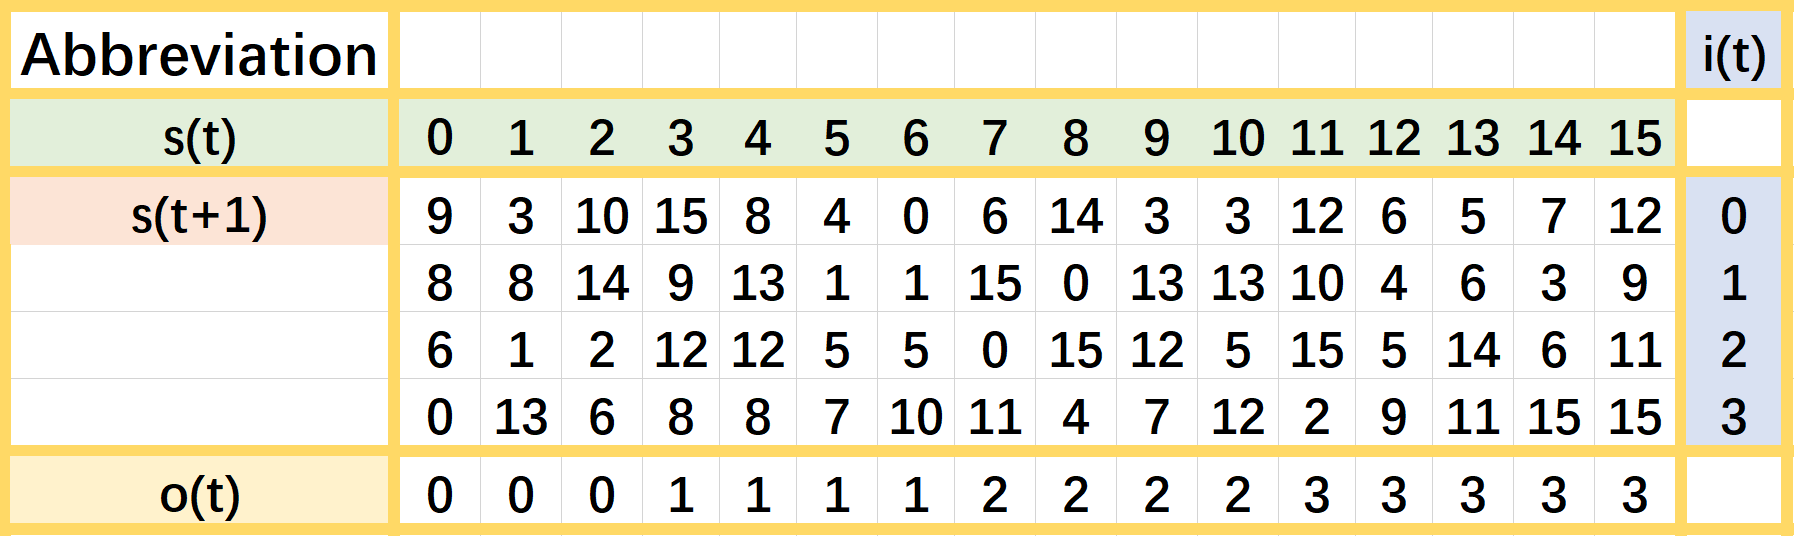
\includegraphics[scale=0.122]{figures/Fig7.png}}
%	}}
%      
%      \caption{The abbreviation form of the updating rules.}
%      \label{fig:6}
%   \end{figure}
%  
%   With the abbreviation forms of $\mathsf{i}(t)$, $\mathsf{s}(t)$ and $\mathsf{o}(t)$, it would be easier for us to use this \BCN\ to explain various concepts by checking this table.
  % 
%For instance, if $\mathsf{s}(t)=\delta^5_{16}$ and $\mathsf{i}(t)=\delta^1_{4}$, then we can know that $\mathsf{s}(t+1)=\delta^4_{16}$  and $\mathsf{s}(t+1)=\delta^1_{4}$ by checking this table.   
 % \tl{(1)simplify later?!} 
%   \begin{itemize}
% \item $\Delta_M = \{\delta^0_{2^m},\ldots,\delta^{({2^m}-1)}_{2^m} \}$ represents the input set; 
% \item $\Delta_N = \{\delta^0_{2^n},\ldots,\delta^{({2^n}-1)}_{2^n} \}$ represents the state set; 
% \item $\Delta_Q = \{\delta^0_{2^q},\ldots,\delta^{({2^q}-1)}_{2^q} \}$ represents the output set,
%\end{itemize}
%where $M=2^m$, $N=2^n$ and $Q=2^q$.
%=======================================================================

%=======================================================================


\subsection{Control theoretical properties of \BCNs}
In this subsection, we introduce the notations controllability, observability and identifiability of {\BCNs} and their relations. 
In particular, we will give a summary about the existing work on observability in order to motivate our work. To this end, first define some notations below.

Given a {\BCN} $\BB = (I,S,O, E, \sigma, \rho,\theta)$, let $\mathcal{I}$, $\mathcal{S}$ and $\mathcal{O}$ be the sets of all possible inputs, states and outputs of $\BB$, respectively. For any $t,t' \in \mathbb{T}$, we define the timed behavior of $\BB$
\begin{itemize}
\item $\mathcal{B}^T = (\mathcal{I}^T, \mathcal{S}^T, \mathcal{O}^T)$,  where 
{\small \[\begin{array}{llll}
\mathcal{I}^T =\{\mathsf{I}[t]~|~ t\in \mathbb{T}, \mathsf{I}[t]=\mathsf{i}(0)\ldots \mathsf{i}(t)\}\\
\mathcal{S}^T =\{\mathsf{S}[t]~|~ t\in \mathbb{T}, \mathsf{S}[t]=\mathsf{s}(0)\ldots \mathsf{s}(t)\}\\
\mathcal{O}^T =\{\mathsf{O}[t]~|~ t\in \mathbb{T}, \mathsf{O}[t]=\mathsf{o}(0)\ldots \mathsf{o}(t)\}\\
\end{array}
\]} such that each for any $\mathsf{s}(k)$ and $\mathsf{o}(k)$ of any $\mathsf{S}[t]$ and 
$\mathsf{O}[t]$ in $\mathcal{S}^T$ and $\mathcal{O}^T$, respectively,   satisfies the updating rules in Definition~\ref{def:BCN}.
%\item Let $\mathsf{S}(t) = \{ \mathsf{s}(t)~|~ \mathsf{s}(0)\ldots \mathsf{s}(t) \in \mathcal{S}^T\}$ and $\mathsf{O}(t) = \{ \mathsf{o}(t)~|~ \mathsf{o}(0)\ldots \mathsf{o}(t) \in \mathcal{O}^T\}$, which do not necessarily have all the possible $2^m$ and $2^n$ as they are generated in the timed behavior according to the updating rules. Note that at any time the input node can take any value in $\mathbb{B}$.
\item For any interval  $[t_0,t]$ of time $\mathbb{T}$, where $t\geq t_0$, we define the following sets 
\[\begin{array}{llllll}
\mathcal{I}^{[t]} &=& \{\mathsf{I}[t] ~|~ \mathsf{I}[t]\in \mathcal{I}^T\}\\
\mathcal{I}^{[t_0,t]} &=& \{\mathsf{i}(t_0)\ldots \mathsf{i}(t)~|\exists \mathsf{i}(0)\ldots \mathsf{i}(t_0)\in \mathcal{I}^{[t_0]}\cdot\\
&& \mathsf{i}(0)\ldots \mathsf{i}(t_0) \ldots \mathsf{i}(t)\in \mathcal{I}^{[t]}\} \\
\mathcal{S}^{[t]} &=& \{\mathsf{S}[t] ~|~ \mathsf{S}[t]\in \mathcal{S}^T\}\\
\mathcal{S}^{[t_0,t]} &=& \{\mathsf{s}(t_0)\ldots \mathsf{s}(t+1)~|\exists \mathsf{s}(0)\ldots \mathsf{s}(t_0)\in \mathcal{S}^{[t_0]}\cdot\\
&& \mathsf{s}(0)\ldots \mathsf{s}(t_0) \ldots \mathsf{s}(t)\in \mathcal{S}^{[t]} \\
\mathcal{O}^{[t]} &=& \{\mathsf{O}[t] ~|~ \mathsf{O}[t]\in \mathcal{O}^T\}\\
\mathcal{O}^{[t_0,t]} &=& \{\mathsf{o}(t)\ldots \mathsf{o}(t_0)~|\exists \mathsf{o}(0)\ldots \mathsf{o}(t_o)\in \mathcal{O}^{[t_0]}\cdot\\
&& \mathsf{o}(0)\ldots \mathsf{o}(t_o) \ldots \mathsf{o}(t)\in \mathcal{O}^{[t]} \}\\
\end{array}
\]
\end{itemize} 
The sets $\mathcal{I}^{[t_0,t]}$, $\mathcal{S}^{[t_0,t]}$ and $\mathcal{O}^{[t_0,t]}$ are the possible inputs, states and outputs of the execution of $\BB$ in the interval $[t_0,t]$ of observing time. 

		We now define the following two functions which define,  for any interval $[t_0,t]$ of observing time from $t_0$ to $t$,  the sequence of states and sequence of outputs produced, respectively,  in the interval by a state $\mathsf{s}(t_0)$ at time $t_0$ and a sequence of inputs in the interval. Formally, the two functions are defined as:


\begin{equation}
\begin{split}
F^{[t_0,t]}&: S(t_0)\times \mathcal{I}^{[t_0,t]} \mapsto \mathcal{S}^{[t_0,t+1]}\\
F^{[t_0,t]}&(\mathsf{s}, \mathsf{i}(t_0)\ldots \mathsf{i}(t))= \mathsf{s}(t_0)\ldots \mathsf{s}(t+1)\\
 \end{split}
\end{equation}
 \begin{equation}
\begin{split}
 H^{[t_0,t]}&: S(t_0)\times \mathcal{I}^{[t_0,t]} \mapsto \mathcal{O}^{[t_0,t+1]}\\
H^{[t_0,t]}&(\mathsf{s}, \mathsf{i}(t_0)\ldots \mathsf{i}(t))= \mathsf{o}(t_0)\ldots \mathsf{o}(t+1)\\
\end{split}
\end{equation}

\[
\begin{array}{llllll}
\mbox{such that the following conditions are satisfied}\\
 (\mathsf{s}(t_0)=\mathsf{s})\wedge \\
 \forall t'=(t_0+1),\ldots,(t+1)\cdot (\mathsf{s}(t')=\sigma(\mathsf{i}(t'-1),\mathsf{s}(t'-1)))\wedge \\
 \forall t'=t_0,\ldots,(t+1)\cdot (\mathsf{o}(t')=\rho(\mathsf{s}(t'))
\end{array}
\]

These functions generalize the two functions given in ~\cite{Zhang2016Observability} for observability,  where only the special case of $F^{[0,t]}$ and $H^{[0,t]}$ are given. The their extensions  will be used when we present the the new observability.
\begin{definition} [Observability~\cite{cheng2009controllability, Zhao2010Input, Cheng2011Identification, Fornasini2013Observability}]
We define the four types of observability below. 
\begin{itemize}
  \item The {\bf Type-I} observability is that, a \BCN\ is observable if for every initial state $\mathsf{s}\in \mathcal{S}$, there exists an input sequence $\mathsf{I}[t]\in\mathcal{I}^{[t]}$ for some $t\in\mathbb{T}$, such that for all states $\mathsf{s}'$, $H^{[0,t]}(\mathsf{s}',\mathsf{I}[t])\neq H^{[0,t]}(\mathsf{s}, \mathsf{I}[t])$ if $\mathsf{s}\ne\mathsf{s}'$.
  \item The  {\bf Type-II} observability is that, a \BCN\ is observable if for every two distinct initial states $\mathsf{s}$ and $\mathsf{s}' \in \mathcal{S}$, there is an input sequence $\mathsf{I}[t]\in\mathcal{I}^{[t]}$ for some $t\in\mathbb{T}$, such that $H^{[0,t]}(\mathsf{s}',\mathsf{I}[t])\neq H^{[0,t]}(\mathsf{s}, \mathsf{I}[t])$.
  \item The {\bf Type-III} observability is that, a \BCN\ is observable if there exists an input sequence $\mathsf{I}[t]\in\mathcal{I}^{[t]}$ for some $t\in\mathbb{T}$, such that for any two distinct states $\mathsf{s}(0)$, $\mathsf{s}'(0) \in \mathcal{S}$, $H^{[0,t]}(\mathsf{s}'(0),\mathsf{I}[t])\neq H^{[0,t]}(\mathsf{s}(0), \mathsf{I}[t])$.
  \item The {\bf Type-IV} observability is that, a \BCN\ is observable, if there is a  natural number $N$, such that for every input sequence $\mathsf{I}[t]\in\mathcal{I}^{[t]}$ with $t\ge N$, $H^{[0,t]}(\mathsf{s}'(0),\mathsf{I}[t])\neq H^{[0,t]}(\mathsf{s}(0), \mathsf{I}[t])$ holds for any two distinct states $\mathsf{s}$, $\mathsf{s}' \in \mathcal{S}$.
\end{itemize} 
\end{definition}

It is noted in ~\cite{Zhang2016Observability} that {\bf Type-I} observability is stronger than {\bf Type-II} observability; {\bf Type-III} observability is stronger than {\bf Type-I} observability;  and while {\bf Type-IV} observability is the strongest. 
%The  {\bf Type-I} observability means that a \BCN\ is observable if every \State$(0)$ of the \BCN\ can be distinguished from other types of initial state by an input sequence $\mathsf{I}[k]$. The {\bf Type-II} observability means that a \BCN\ is observable if for every two distinct $\mathsf{s}(0)$, $\mathsf{s}'(0)$, there is an input sequence $\mathsf{I}[k]$ which distinguishes them.
 %The {\bf Type-III} observability means that a \BCN\ is called observable if there exists an input sequence $\mathsf{I}[k]$ which determine the $\mathsf{s}(0)$ of the \BCN\ for every $\mathsf{s}(0)\in\mathcal{S}$, because $\mathsf{I}[k]$ can distinguish all distinct initial states. The {\bf Type-IV} observability means that a \BCN\ is observable if every sufficient long $\mathsf{I}[k]$ can determine the $\mathsf{s}(0)$ of the \BCN\ for every $\mathsf{s}(0)\in\mathcal{S}$.


 %Thus, we can only check whether $\mathsf{s}(0)=\mathsf{s}^{x}(0)$ or not by $\mathsf{I}^x$. %
%\begin{example}
%For example, for the \BCN\ mentioned in {\em Example \ref{exa:2}}, we have every \State$(0)$ can be distinguished from other types of initial state by an $\mathsf{I}[k] \in(\mathcal{I})^k$.  For instance,
%\begin{itemize}
%  \item $\delta_{16}^0$ can be distinguished from other types of initial state by any $\mathsf{I}[k]$ with the prefix $\delta_{4}^3$, $\delta_{4}^2$ or $\delta_{4}^0  \delta_{4}^2$;%
%  \item $\delta_{16}^1$ can be distinguished from other types of initial state by any $\mathsf{I}[k]$ with the prefix $\delta_{4}^0$, $\delta_{4}^3$ or $\delta_{4}^2 \delta_{4}^3$;
 % \item $\delta_{16}^2$ can be distinguished from other types of initial state by any $\mathsf{I}[k]$ with the prefix $\delta_{4}^1$, $\delta_{4}^3$ or $\delta_{4}^0 \delta_{4}^2$, etc.
%\end{itemize} 
%Therefore, this \BCN\ satisfies the  {\bf Type-I} observability.
%\label{exa:4}
%\end{example}   

%\begin{definition}[ {\bf Type-II} Observability~\cite{Zhao2010Input}]
%	The  {\bf Type-II} observability is that, a \BCN\ is observable if for every two distinct initial states $\mathsf{s}(0)$, $\mathsf{s}'(0) \in \mathcal{S}$, there is an input sequence $\mathsf{I}[k]\in(\mathcal{I})^k$ for some $k>0$, such that $\rho(\mathsf{s}(0))=\rho(\mathsf{s}'(0))$ implies $(HF)^k_{\mathsf{s}(0)}(\mathsf{I}[k])\neq (HF)^k_{\mathsf{s}'(0)}(\mathsf{I}[k])$.
%\end{definition}

 %Therfore, we can only check $\mathsf{s}(0)=\mathsf{s}^{x}(0)$ or $\mathsf{s}(0)=\mathsf{s}^{y}(0)$ when we know that $\mathsf{s}(0)$ is one of them by $\mathsf{I}^{xy}$. 
%\begin{example}
%For example, for the \BCN\ mentioned in {\em Example \ref{exa:2}}, we have for every two distinct $\mathsf{s}(0)$ and $\mathsf{s}'(0)$, there exists an $\mathsf{I}[k]\in(\mathcal{I})^k$ which distinguishes them.  For instance,
%\begin{itemize}
 % \item $\mathsf{I}[k]$ with the prefix $\delta_{4}^0$ can distinguish $\delta_{16}^0$ and $\delta_{16}^1$;
 % \item $\mathsf{I}[k]$ with the prefix $\delta_{4}^1$ can distinguish $\delta_{16}^0$ and $\delta_{16}^2$;
 % \item $\mathsf{I}[k]$ with the prefix $\delta_{4}^3$ can distinguish $\delta_{16}^1$ and $\delta_{16}^2$.
%\end{itemize} 
%Therefore this \BCN\ satisfies the {\bf Type-II} observability.
%\label{exa:5}
%\end{example}   
%\begin{definition}[{\bf Type-III} Observability~\cite{Cheng2011Identification}]
%The {\bf Type-III} observability is that, a \BCN\ is observable if there exists an input sequence $\mathsf{I}[k]\in(\mathcal{I})^k$ for some $k>0$, such that for any two distinct states $\mathsf{s}(0)$, $\mathsf{s}'(0) \in \mathcal{S}$, $\rho(\mathsf{s}(0))=\rho(\mathsf{s}'(0))$ implies $(HF)^k_{\mathsf{s}(0)}(\mathsf{I}[k])\neq (HF)^k_{\mathsf{s}'(0)}(\mathsf{I}[k])$.
%\end{definition}

%, the $\mathsf{s}(0)$ is determined by its corresponding output sequence $(HF)^k_{\mathsf{s}(0)}(\mathsf{I})$.

%\begin{example}
%For example, for the \BCN\ mentioned in {\em Example \ref{exa:2}}, for any $k>0$, there is not an $\mathsf{I}[k]\in(\mathcal{I})^k$ which determines the $\mathsf{s}(0)$ of this \BCN:
%\begin{itemize}
 % \item $\mathsf{I}[k]$ with prefix $\delta_{4}^0$ can not distinguish $\delta_{16}^9$ and $\delta_{16}^{10}$;
%  \item $\mathsf{I}[k]$ with prefix $\delta_{4}^1$ can not distinguish $\delta_{16}^0$ and $\delta_{16}^{1}$;
%  \item $\mathsf{I}[k]$ with prefix $\delta_{4}^2$ can not distinguish $\delta_{16}^3$ and $\delta_{16}^{4}$;
 % \item $\mathsf{I}[k]$ with prefix $\delta_{4}^3$ can not distinguish $\delta_{16}^{14}$ and $\delta_{16}^{15}$.
%\end{itemize} 
%Therefore it does not satisfy the {\bf Type-III} observability. 
%\label{exa:6}
%\end{example}  
%\begin{definition}[{\bf Type-IV} Observability~\cite{Fornasini2013Observability}]
%	The {\bf Type-IV} observability is that, a \BCN\ is observable, if there is a  natural number $N$, such that for every input sequence $\mathsf{I}[k]\in(\mathcal{I})^{k}$, for any two distinct states $\mathsf{s}(0)$, $\mathsf{s}'(0) \in \mathcal{S}$, $\rho(\mathsf{s}(0))=\rho(\mathsf{s}'(0))$ implies $(HF)^{k}_{\mathsf{s}(0)}(\mathsf{I}[k])\neq (HF)^{k}_{\mathsf{s}'(0)}(\mathsf{I}[k])$ if  $k\ge N$.
%\end{definition}

%, because every sufficient long $\mathsf{I}[k]$ can distinguish any two distinct initial states.%, the $\mathsf{I}$ can be determined by its output sequence $(HF)^k_{\mathsf{s}(0)}(\mathsf{I})$.
%\begin{example}
%For example, for the \BCN\ mentioned in {\em Example \ref{exa:2}}, any $\mathsf{I}[k]$ with prefix $\delta_{4}^0$ can not can not distinguish $\delta_{16}^9$ and $\delta_{16}^{10}$. 
%Therefore this \BCN\ does not satisfy the {\bf Type-IV} observability. 
%\label{exa:7}
%\end{example}  

%The implication relationships of four existing types of observability is that, {\bf Type-I} observability is stronger than {\bf Type-II} observability, {\bf Type-III} observability is stronger than {\bf Type-I} observability and {\bf Type-II} observability, while {\bf Type-IV} observability is strongest~\cite{Zhang2016Observability}. If a \BCN\ satisfies {\bf Type-I} observability, then for every initial state $\mathsf{s}(0)$ there exists an input sequence $\mathsf{I}[t]$ which can distinguish $\mathsf{s}(0)$ from other initial states, and then in this \BCN, for every two distinct initial states $\mathsf{s}(0)$, $\mathsf{s}'(0) $ there exists an input sequence $\mathsf{I}'[t]$ which can distinguish them, thus it satisfies {\bf Type-II} observability. Therefore, {\bf Type-I} observability is stronger than {\bf Type-II} observability. If a \BCN\ satisfies {\bf Type-III} observability, then there exists an input sequence $\mathsf{I}[t]$ which can distinguish every two distinct initial states $\mathsf{s}(0)$, $\mathsf{s}'(0)$, and then in this \BCN, for every initial state $\mathsf{s}(0)$ the input sequence $\mathsf{I}[t]$ can distinguish $\mathsf{s}(0)$ from other initial states, thus it satisfies {\bf Type-II} observability. Therefore, {\bf Type-III} observability is stronger than {\bf Type-I} observability and {\bf Type-II} observability. If a \BCN\ satisfies {\bf Type-IV} observability, then every sufficient long input sequence $\mathsf{I}[t]$ can distinguish every two distinct initial states $\mathsf{s}(0)$, $\mathsf{s}'(0)$, thus it satisfies {\bf Type-III} observability too. Therefore, {\bf Type-IV} observability is strongest. 

% \begin{figure}[thpb]
   %  \centering
 %   \framebox{\parbox{3in}{
%		\centerline{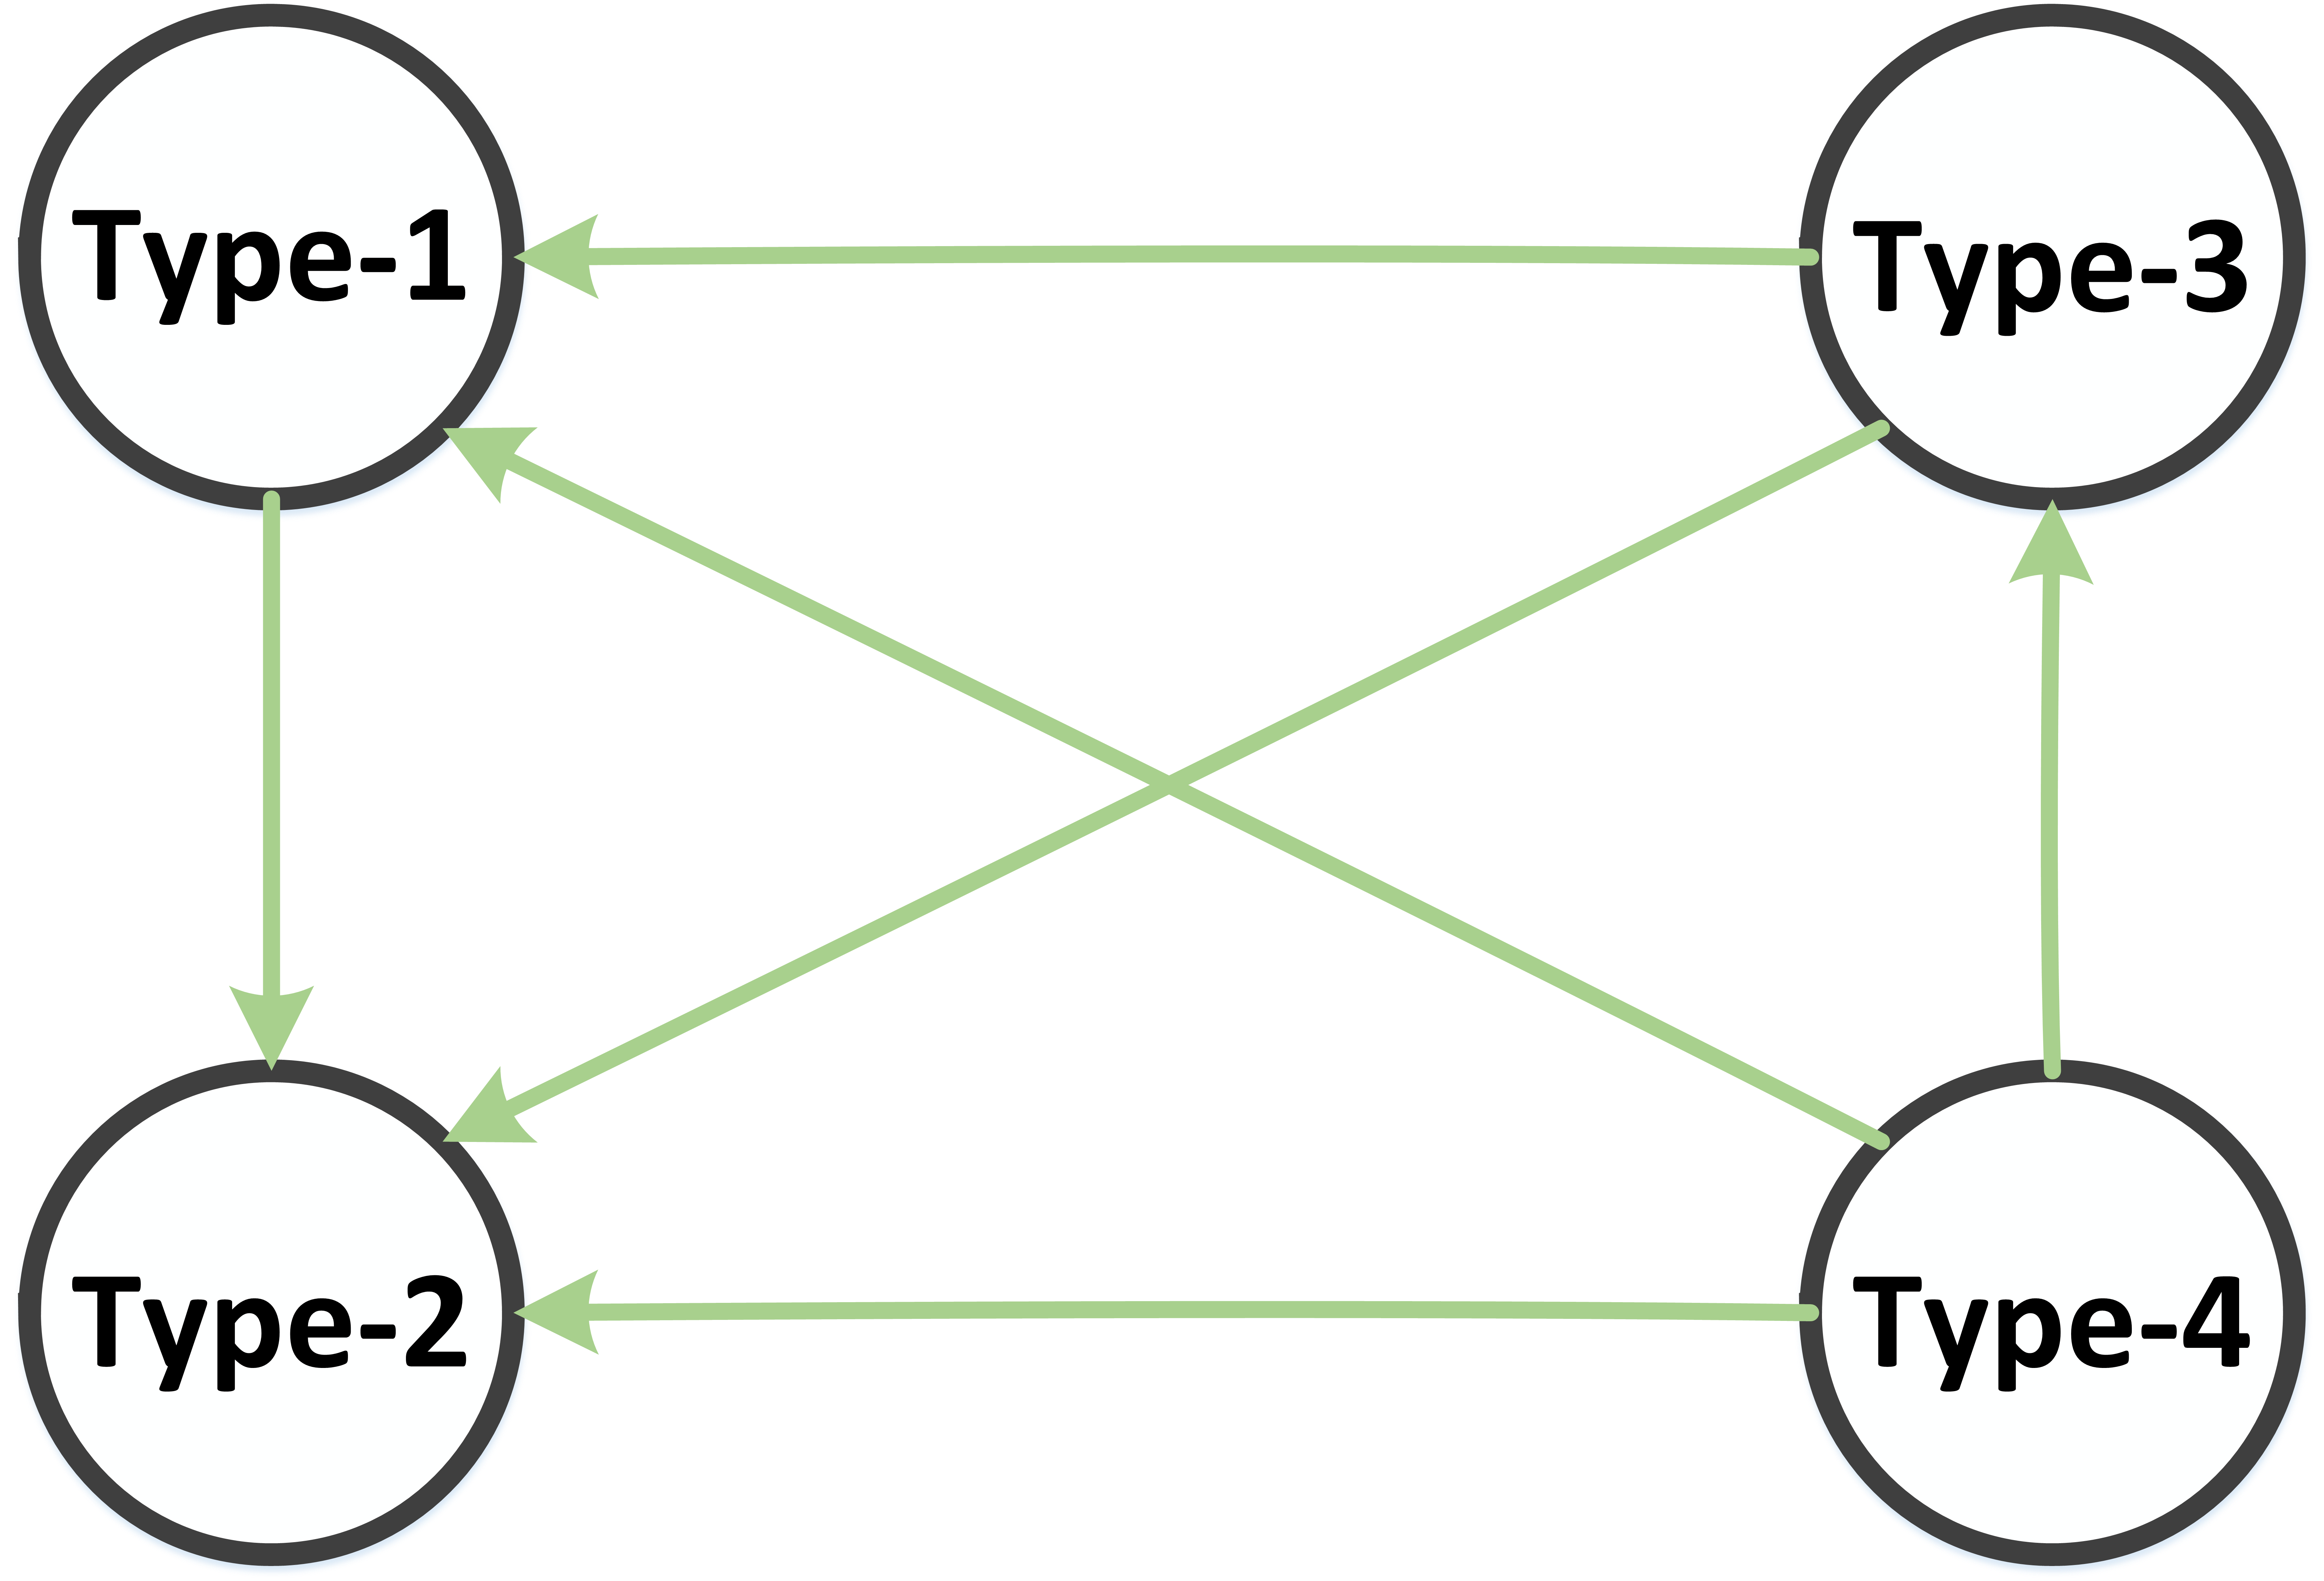
\includegraphics[scale=0.27]{figures/Fig9.png}}
%	}}
      
   %  \caption{The implication relationships graph between observability {\bf Type-I}, {\bf Type-II}, {\bf Type-III} and {\bf Type-IV}, where ``$\rightarrow$" means ``implies".}
%      \label{fig:9}
  % \end{figure}

%The implication relationship is that ``The first observability implies the second observability.'' means ``If a \BCN\ satisfies the first observability, then it satisfies the second observability.'' 



%\subsection{Controllability and identifiability of \BCNs}
%\tl{what's the point here?}


\begin{definition}[Controllability~\cite{cheng2009controllability}]
	A \BCN\ is controllable if for any two distinct states $\mathsf{s}$, $\mathsf{s}' \in \mathcal{S}$, there is an input sequence $\mathsf{I}[t]\in\mathcal{I}^{[t]}$,  for some $t\in\mathbb{T}$, such that  $F^{[0,t]}(\mathsf{s}, \mathsf{I}[t])=\mathsf{s}(0) \ldots\, \mathsf{s}(t+1)$ and the last state  $\mathsf{s}(t+1)$ is $\mathsf{s}'$.
\end{definition}

Thus, if a \BCN\  $\BB$ is  controllable,  any state $\mathsf{s}'$ is reachable from an initial state $\mathsf{s}$, and  we use an input  sequence $\mathsf{I}[t]$ make $\BB$ reach $\mathsf{s}'$ from $\mathsf{s}$.
%\begin{example}
%For example, the \BCN\ mentioned in {\em Example \ref{exa:2}} is controllable, that is for any initial state $\mathsf{s}(0)$ and destination state $\mathsf{s}'$, there is an input sequence $\mathsf{I}[k]$, such that in the $F^k_{\mathsf{s}(0)}(\mathsf{I}[k])=\mathsf{s}(1) \ldots\, \mathsf{s}(k)$, the $\mathsf{s}(k)=\mathsf{s}'$. For instance, for the initial state $\mathsf{s}(0)= \delta_{16}^{1}$ and destination state $\mathsf{s}'=\delta_{16}^{2}$, there is an input sequence $\mathsf{I}[3]=\delta_{4}^{3}\delta_{4}^{3}\delta_{4}^{3}$, such that $F^3_{\mathsf{s}(0)}(\delta_{4}^{3}\delta_{4}^{3}\delta_{4}^{3})=\delta_{16}^{13}\delta_{16}^{11}\delta_{16}^{2}$.
%\label{exa:12}
%\end{example}  

\begin{definition}[Identifiability~\cite{Cheng2011Identification}]%
A \BCN\ is identifiable if  there exists an input sequence $\mathsf{I}[t]\in\mathcal{I}^{[t]}$ for some $t \in \mathbb{T}$ such that the updating rules
	\begin{equation*}
    		\begin{split}
		\mathsf{s}(t+1)=&\sigma(\mathsf{i}(t),\mathsf{s}(t))\\
		\mathsf{o}(t)=&\rho(\mathsf{s}(t))
		\end{split}
	\end{equation*}
	can be constructed by the input  sequence  $\mathsf{I}[t]$ and its corresponding output sequence  $\mathsf{O}[t+1]$. 
\end{definition}

Thus, a \BCN\  $\BB$ is identifiable if the updating functions $\sigma$ and $\rho$ can be uniquely determined by a  designed input sequence  $\mathsf{i}(0)\ldots \mathsf{i}(t)$.

%\begin{definition}[Observability]
%A \BCN\ $\BB$ is observable if there exists an input sequence $\mathsf{I}\in(\Delta_L)^k$ for some $k>0$, such that for any two distinct states $\mathsf{s}(0)$, $\mathsf{s}'(0) \in \Delta_M$, $h(\mathsf{s}(0))=h(\mathsf{s}'(0))$ implies $(HF)^k_{\mathsf{s}(0)}(\mathsf{I})\neq (HF)^k_{\mathsf{s}'(0)}(\mathsf{I})$ \cite{Cheng2011Identification}.
%\end{definition}

%The observability means that a \BCN\ is called observable if there exists an input sequence $\mathsf{I}\in(\Delta_L)^k$ which determine the $\mathsf{s}(0)$ of the \BCN\ for every $\mathsf{s}(0)\in\Delta_M$, because $\mathsf{I}$ can distinguish any two distinct initial states.%, the $\mathsf{s}(0)$ is determined by its corresponding output sequence $(HF)^k_{\mathsf{s}(0)}(\mathsf{I})$.

%\begin{example}
%For example, for the \BCN\ mentioned in {\em Example \ref{exa:2}}, for any $k>0$, there is not any $\mathsf{I}\in(\Delta_L)^k$ which can determine the $\mathsf{s}(0)$ of this \BCN:
%\begin{itemize}
 % \item any $\mathsf{I}$ with prefix $\delta_{4}^0$ can not distinguish $\delta_{16}^9$ and $\delta_{16}^{10}$;
 % \item any $\mathsf{I}$ with prefix $\delta_{4}^1$ can not distinguish $\delta_{16}^0$ and $\delta_{16}^{1}$;
  %\item any $\mathsf{I}$ with prefix $\delta_{4}^2$ can not distinguish $\delta_{16}^3$ and $\delta_{16}^{4}$;
%  \item any $\mathsf{I}$ with prefix $\delta_{4}^3$ can not distinguish $\delta_{16}^{14}$ and $\delta_{16}^{15}$.
%\end{itemize} 
%Therefore it does not satisfy the observability. 
%\label{exa:6}
%\end{example}  

The properties of observability, controllability and identifiability are closely related. In particular, it is proven in~\cite{Cheng2011Identification} that a \BCN\ is identifiable iff  it is controllable and its initial state can be determined through experiments with input sequences without the need of (or without knowing the mechanism for) resetting the initial state. Furthermore in ~\cite{Cheng2011Identification}, it states that the observability of  {\bf Type-III}  is both sufficient and necessary for determining the initial state of a \BCN\  without  resetting.  

However, we discover there are some \BCNs\ which do not satisfy the {\bf Type-III} but their initial states can be determined without resetting. 

For instance, in the \BCN\ in {\em Example \ref{exa:2}}, for any $t\in \mathbb{T}$, there is not an $\mathsf{I}[t]\in\mathcal{I}^{[t]}$ which can distinguish every two distinct initial states $\mathsf{s}$, $\mathsf{s}'$. Because for any $t\in \mathbb{T}$,%For example, any input sequence $\mathsf{I}[t]$ starting with the input $(00)$ can not distinguish the distinct states $(1001)$ and $(1010)$, because 
\begin{itemize}
\item for any $\mathsf{I}[t]$ starting with $\mathsf{i}^0$, $H^{[0,t]}(\mathsf{s}^9,\mathsf{I}[t])= H^{[0,t]}(\mathsf{s}^{10}, \mathsf{I}[t])$;
  \item for any $\mathsf{I}[t]$ starting with $\mathsf{i}^1$, $H^{[0,t]}(\mathsf{s}^0,\mathsf{I}[t])= H^{[0,t]}(\mathsf{s}^1, \mathsf{I}[t])$;
  \item for any $\mathsf{I}[t]$ starting with $\mathsf{i}^2$, $H^{[0,t]}(\mathsf{s}^3,\mathsf{I}[t])= H^{[0,t]}(\mathsf{s}^4, \mathsf{I}[t])$;
  \item for any $\mathsf{I}[t]$ starting with $\mathsf{i}^3$, $H^{[0,t]}(\mathsf{s}^{14},\mathsf{I}[t])= H^{[0,t]}(\mathsf{s}^{15}, \mathsf{I}[t])$.
\end{itemize} 
%Therefore it does not satisfy the {\bf Type-III} observability. 
Therefore it does not satisfy the {\bf Type-III} observability. But in this \BCN,%, thus we can determine the initial state of it even if its initial state can not be reset. And this \BCN\ is controllable, thus it is identifiable.  %Thus with the online observability we can research the \BCNs\ better.

\begin{itemize}
  \item we can classify all states into four sets by their corresponding outputs, that 
  \begin{itemize}
   \item for any $\mathsf{s}\in\{\mathsf{s}^0,\mathsf{s}^1,\mathsf{s}^2\}$, $\rho(\mathsf{s})=\mathsf{o}^0$;
   \item for any $\mathsf{s}\in\{\mathsf{s}^3,\mathsf{s}^4,\mathsf{s}^5,\mathsf{s}^6\}$,  $\rho(\mathsf{s})=\mathsf{o}^1$;
   \item for any $\mathsf{s}\in\{\mathsf{s}^7,\mathsf{s}^8,\mathsf{s}^9,\mathsf{s}^{10}\}$,  $\rho(\mathsf{s})=\mathsf{o}^2$;
   \item for any $\mathsf{s}\in\{\mathsf{s}^{11},\mathsf{s}^{12},\mathsf{s}^{13},\mathsf{s}^{14},\mathsf{s}^{15}\}$, $\rho(\mathsf{s})=\mathsf{o}^3$.
  \end{itemize} 
    
  \item For the $\mathsf{I}[t]=\mathsf{i}^3$, for every two distinct initial states $\mathsf{s}$, $\mathsf{s}'\in \{\mathsf{s}^0,\mathsf{s}^1,\mathsf{s}^2\}$,  $H^{[0,t]}(\mathsf{s}',\mathsf{I}[t])\neq H^{[0,t]}(\mathsf{s}, \mathsf{I}[t])$, where $t=0$;
  \item For the  $\mathsf{I}[t]=\mathsf{i}^0$, for every two distinct initial states $\mathsf{s}$, $\mathsf{s}'\in \{\mathsf{s}^3,\mathsf{s}^4,\mathsf{s}^5, \mathsf{s}^5\}$,  $H^{[0,t]}(\mathsf{s}',\mathsf{I}[t])\neq H^{[0,t]}(\mathsf{s}, \mathsf{I}[t])$, where $t=0$;  
  \item For the $\{\mathsf{s}^7,\mathsf{s}^8,\mathsf{s}^9,\mathsf{s}^{10}\}$, we can classify the states belonging to it into three sets by the outputs of $\sigma (\mathsf{i}^3,\mathsf{s}^8)$, $\sigma (\mathsf{i}^3, \mathsf{s}^9)$, $\sigma (\mathsf{i}^3, \mathsf{s}^7)$ and $\sigma (\mathsf{i}^3, \mathsf{s}^{10})$, that  
   \begin{itemize}
   \item  for any $\mathsf{s}\in\{\mathsf{s}^8\}$, $\rho(\sigma (\mathsf{i}^3,\mathsf{s}))=\mathsf{o}^1$;
   \item  for any $\mathsf{s}\in\{\mathsf{s}^9\}$, $\rho(\sigma (\mathsf{i}^3,\mathsf{s}))=\mathsf{o}^2$;
   \item  for any $\mathsf{s}\in\{\mathsf{s}^7,\mathsf{s}^{10}\}$, $\rho(\sigma (\mathsf{i}^3,\mathsf{s}))=\mathsf{o}^3$.
   \end{itemize} 

 
  And for the $\mathsf{I}[t]=\mathsf{i}^3$, for every two distinct initial states $\mathsf{s}$, $\mathsf{s}'\in \{\sigma (\mathsf{i}^3, \mathsf{s}^7),\sigma (\mathsf{i}^3, \mathsf{s}^{10})\}$ the $\{\mathsf{s}^7,\mathsf{s}^{10}\}$, $H^{[0,t]}(\mathsf{s}',\mathsf{I}[t])\neq H^{[0,t]}(\mathsf{s}, \mathsf{I}[t])$, where $t=0$.
  
  \item For the $\{\mathsf{s}^{11},\mathsf{s}^{12},\mathsf{s}^{13},\mathsf{s}^{14},\mathsf{s}^{15}\}$, we can classify the states belonging to it into two sets  by the outputs of $\sigma (\mathsf{i}^1,\mathsf{s}^{11})$, $\sigma (\mathsf{i}^1, \mathsf{s}^{12})$, $\sigma (\mathsf{i}^1, \mathsf{s}^{13})$, $\sigma (\mathsf{i}^1, \mathsf{s}^{14})$ and $\sigma (\mathsf{i}^1, \mathsf{s}^{15})$, that  
    \begin{itemize}
     \item  for any $\mathsf{s}\in\{\mathsf{s}^{11}, \mathsf{s}^{15}\}$, $\rho(\sigma (\mathsf{i}^1,\mathsf{s}))=\mathsf{o}^2$;
   \item  for any $\mathsf{s}\in\{\mathsf{s}^{12},\mathsf{s}^{13},\mathsf{s}^{14}\}$, $\rho(\sigma (\mathsf{i}^1,\mathsf{s}))=\mathsf{o}^1$.
  \end{itemize}
  And 
  \begin{itemize}
   \item for the $\mathsf{I}[t]=\mathsf{i}^2$, for every two distinct initial states $\mathsf{s}$, $\mathsf{s}'\in \{\sigma (\mathsf{i}^1, \mathsf{s}^{11}),\sigma (\mathsf{i}^1, \mathsf{s}^{15})\}$,  $H^{[0,t]}(\mathsf{s}',\mathsf{I}[t])\neq H^{[0,t]}(\mathsf{s}, \mathsf{I}[t])$, where $t=0$;
  \item  for the $\mathsf{I}[t]=\mathsf{i}^0$, for every two distinct states $\mathsf{s}$, $\mathsf{s}'\in \{\sigma (\mathsf{i}^1,\mathsf{s}^{12}),\sigma (\mathsf{i}^1, \mathsf{s}^{13}), \sigma (\mathsf{i}^1, \mathsf{s}^{14})\}$, $H^{[0,t]}(\mathsf{s}',\mathsf{I}[t])\neq H^{[0,t]}(\mathsf{s}, \mathsf{I}[t])$, where $t=0$.
  \end{itemize}
\end{itemize} 
Thus we can determine the initial state of this \BCN\ by its outputs and inputs without resetting the initial state. For instance, when $\mathsf{s}(0)=\mathsf{s}^{15}$, from the output $\mathsf{o}(0)=\mathsf{o}^3$ we have $\mathsf{s}(0)\in \{\mathsf{s}^{11},\mathsf{s}^{12},\mathsf{s}^{13},\mathsf{s}^{14},\mathsf{s}^{15}\}$, then we can input $\mathsf{i}(0)=\mathsf{i}^1$. From the output $\mathsf{o}(1)=\mathsf{o}^2$ we have $\mathsf{s}(0)\in\{\mathsf{s}^{11},\mathsf{s}^{15}\}$, and then we input $\mathsf{i}(1)=\mathsf{i}^2$, such that we determine $\mathsf{s}(0)=\mathsf{s}^{15}$ by the output $\mathsf{o}(2)=\mathsf{o}^3$. In this procedure, we do not need to reset the initial state. And even if the $\mathsf{s}(0)$ with other values, we can determine it by similar procedure without resetting the initial state.



Therefore we find the observability of  {\bf Type-III}  is sufficient but {\bf not necessary} for its initial state being determined without resetting. And the propose a new type of observability named online observability to present the sufficient and necessary condition for determining the initial state of a \BCN\  without  resetting.
%, because the initial state $\mathsf{s}(0)$ of a \BCN\ $\BB$ can be determined by the algorithm (mentioned in {\em Section \ref{sec:intro}}) corresponding to {\bf Type-III} observability when $\BB$ satisfies the {\bf Type-III} observability.


   
% Because we do not make full use of the output and input in the process of determining the initial state. The output of \BCNs\ we observe at every time step can help us further determine the range of the initial state. With the range of the initial state, we can use different input sequence to determine the initial state. While in the third and fourth existing observability, we use the same input sequence $\mathsf{I}$ to determine the initial state.

 
%However, in some biological systems which depicted by \BCNs, the initial states of them can be checked at most once. Therefore,
%The {\bf Type-I} observability and {\bf Type-II} observability are designed to determine the initial states of \BCNs\ when their initial state can be reset. The {\bf Type-IV} observability is designed to study the reconstructibility of \BCN. The {\bf type-III} observability is proposed to research the identification of \BCNs. In this paper, we want to use the new observability we propose to replace the {\bf Type-III} observability, such that we can research the identification problem better.
%As the first observability and second observability are designed to determine the initial states of \BCNs\ by taking the determining procedure multiple times in parallel. %\tl{why this claim?} 
%And in some applications, we have to determine \BCNs' initial states by taking the determining procedure once. The third and fourth observability are designed to determine the initial states of \BCNs\ by taking the determining procedure once. But if a \BCN\ is not satisfy the third observability, we can not use them to determine its initial states by taking the determining procedure once.  %Thus, we propose the online observability of \BCNs\ to solve the problem.
%Moreover, in some biological systems, it would takes many costs to check these biological systems. Hence it would cost a lot of overhead for us to determine the initial state of them by the first observability and second observability.





% \begin{problem}
%\label{pro:2}
%What is the necessary and sufficient condition of determining a \BCN's initial state $\mathsf{s}(0)$ by taking the determining procedure once?
%\end{problem}

